\section{Cơ sở lý thuyết}
\subsection{Thiết kế màn chơi}
\hspace*{1cm} Một màn chơi là không gian những gì cốt lõi diễn ra trong game. Nơi này đặt ra những giới hạn cho người chơi trong việc tương tác với game. Có sự đa dạng trong từng level. Mỗi level có thể có một số điểm tương đồng, nhưng mỗi màn sẽ có những nét đặc trưng khác nhau.\\
\hspace*{1cm} Thiết kế màn chơi là một giai đoạn của quá trình phát triển trò chơi nơi các nhà phát triển tập trung tạo ra các không gian này, bao gồm các cấp độ, bản đồ và nhiệm vụ trong game. Việc thiết kế trò chơi là việc kết hợp các yếu tố cấu thành nên trải nghiệm người chơi, bao gồm cơ chế game, gameplay, cốt truyện,...\\
\hspace*{1cm} Tuy nhiên, việc thiết kế màn chơi không phải để cho có. Việc thiết kế màn chơi cần có một mục đích nào đó, ví dụ như kể chuyện, có nhân vật và phục vụ cho mục đích rõ ràng trong game. Hơn hết, người thiết kế phải tập trung vào trải nghiệm người chơi, hơn là cảm nhận bản thân. Và màn chơi phải thực sự cuốn hút và vui để mang đến trải nghiệm cho người chơi\\
\hspace*{1cm} Mục tiêu của việc thiết kế màn chơi là tạo ra các sự kiện tương tác trong môi trường game sao cho chúng mang tính thử thách người chơi. Giúp người chơi đạt được cảm giác vui sướng khi hoàn thành và có mong muốn tiếp tục gắn bó với game.\\
\subsubsection{Các bước thiết kế một màn chơi}
\hspace*{1cm} Để thiết kế màn chơi, cần tập trung vào các bước chính sau:
\begin{enumerate}
	\item \textbf{Xác định lại giới hạn dự án}\\
	Các ý tưởng có thể có rất nhiều, trông chúng có thể rất hay nhưng mà ta cũng nên nhìn lại xem giới hạn của dự án có phù hợp cho ý tưởng này không, từ đó chọn được các ý tưởng phù hợp. Nó có thể đến từ bản chất của dự án hoặc kỹ thuật. Người thiết kế màn chơi cần hiểu rõ các giới hạn này để thiết kế màn chơi sao cho hợp lý.\\
	\hspace*{1cm} Về bản chất của dự án. Điều cần phải chú ý nhất là người chơi cũng như nền tảng hiện thực. Ta cần xác định đối tượng người chơi chủ đạo của game (là trẻ em, người trưởng thành hay người cao tuổi, là nam hay nữ, có phải là mẹ bỉm sữa hay không,...) cũng như nền tảng để chơi (mobile, PC hay console). Điều này ảnh hưởng đến thời gian hoàn thiện, độ dài và độ khó của màn chơi cũng như phong cách đồ hoạ. Những dự án làm trên mobile sẽ nhanh hơn so với PC hay console. Những trò chơi nhắm đến đối tượng trẻ em thì độ dài màn chơi sẽ ngắn, độ khó cũng dễ hơn cũng như phong cách đồ hoạ cũng sẽ nhẹ đô hơn so với các game dành cho lứa tuổi người trưởng thành. Ta không thể sản xuất một tựa game có phong cách đồ hoạ máu me, hoặc chủ đề có liên quan đến chiến tranh cho đối tượng là trẻ em được.\\
	\hspace*{1cm} Về vấn đề kỹ thuật, người thiết kế màn chơi phải giữ cho game có tính nhất quán về mặt công nghệ. Người thiết kế cần biết dự án sẽ sử dụng công nghệ nào, phong cách đồ hoạ ra sao, âm thanh, nhạc nền như thế nào. Một trò chơi không thể sử dụng lẫn lộn đồ hoạ pixel và đồ hoạ vector nếu không có mục đích cụ thể, hoặc có mục đích nhưng sử dụng không hợp lý. Một trò chơi về chiến tranh thế giới thời hiện đại không thể xuất hiện các yếu tố như pháp sư, phù thuỷ hay kiếm sĩ trong các tựa game RPG được. Ngược lại, một trò chơi RPG Fantasy nếu không có yếu tố liên quan đến thế giới thực thì không thể nào có thứ gọi là súng được. Ngoài ra  Ngoài ra, hiệu ứng ánh sáng và môi trường trong game cũng là một vấn đề đáng lưu tâm. Ở các tựa game kinh dị hù doạ hoặc truy đuổi, môi trường và ánh sáng sẽ tác động nhiều đến cảm xúc của người chơi, có thể tạo cho người chơi cảm giác hồi hộp, thót tim nếu sử dụng hợp lý.\\
	\hspace*{1cm} Dưới đây là một game có thiết kế màn chơi có vấn đè về kỹ thuật, trong việc sử dụng cả pixel art, vector art và hiệu ứng ánh sáng chưa hợp lý.\\
	\begin{figure}[H]
		\centering
		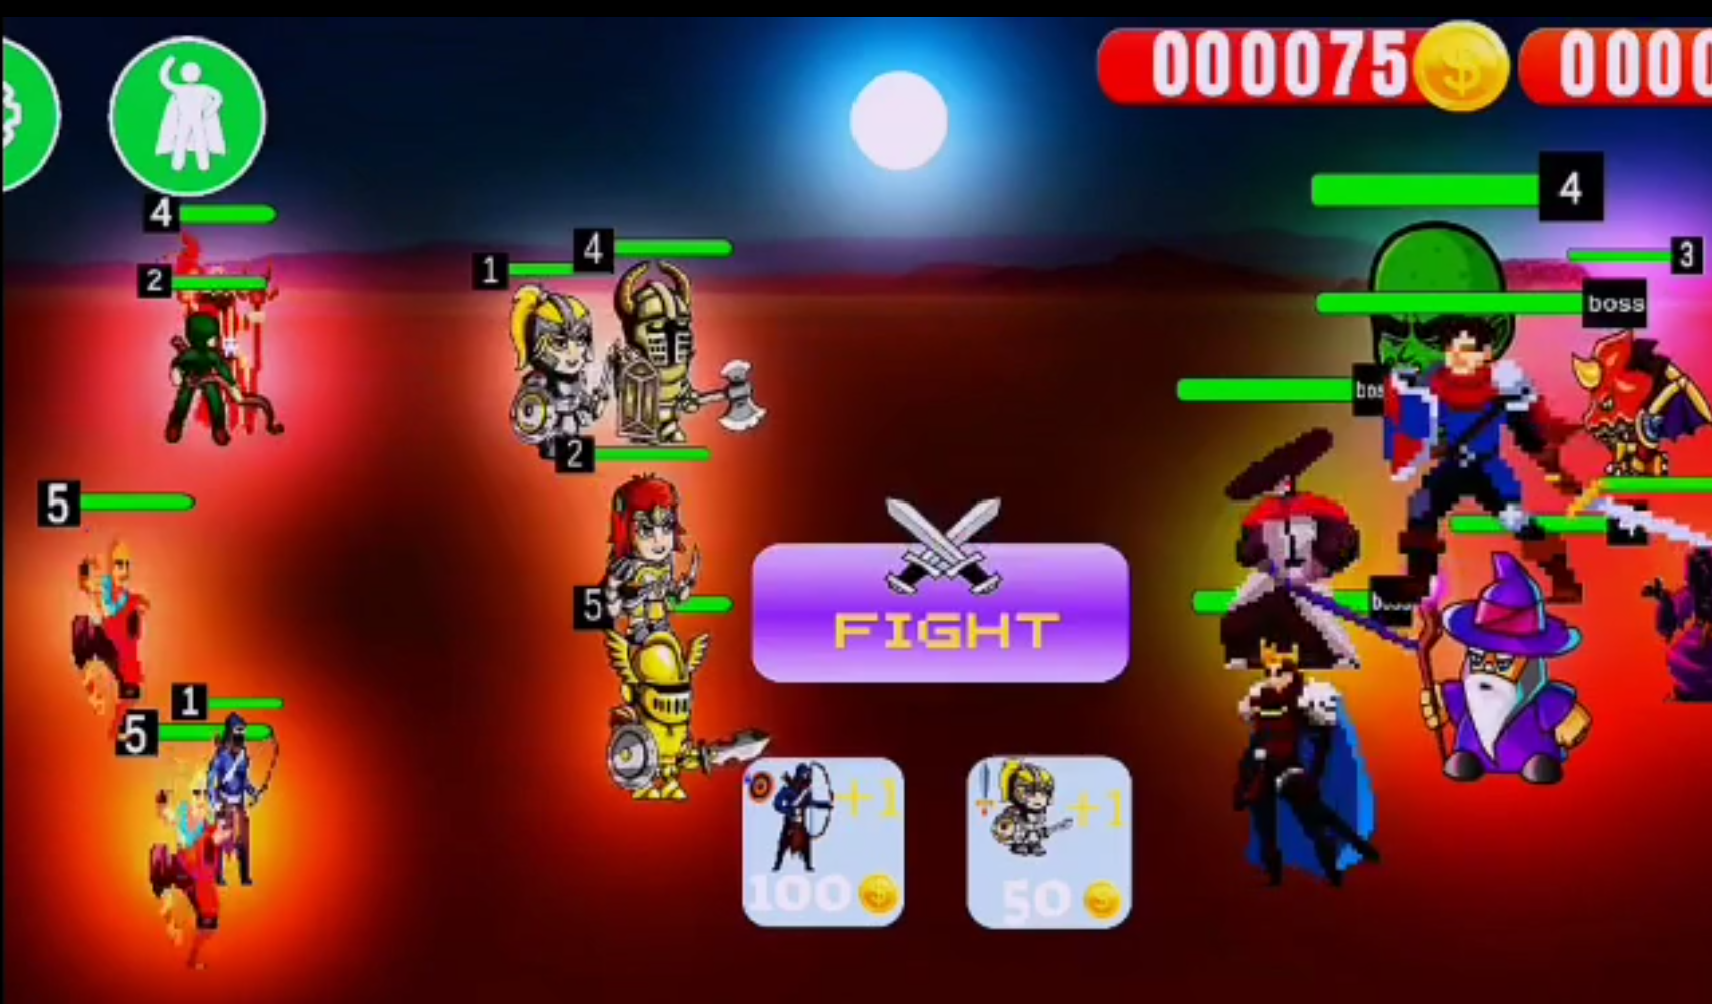
\includegraphics[width=\textwidth]{Images/AGameSuck.png}
		\vspace{0.5cm}
		\caption{Một màn chơi của game gặp vấn đề về kỹ thuật}
	\end{figure}

	\item \textbf{Lên ý tưởng và phác hoạ sơ bộ cấu trúc.}\\
	\hspace*{1cm}  Ở giai đoạn này, các thành viên khác trong dự án sẽ tiến hành lên ý tưởng và phác hoạ lên diẽn biến chính của cốt truyện cũng như xác định sơ bộ các thành phần khác của trò chơi như hình ảnh, âm thanh. Để việc thiết kế được dễ dàng hơn, người thiết kế có thể chia màn chơi thành các zone nhỏ sao cho dễ quản lý. Người thiết kế nên nghĩ đến màn chơi nếu chia thành nhiều zone sẽ ra sao và thiết kế từng zone riêng biệt để đạt hiệu suất cao và đơn giản hơn so với thiết kế toàn bộ màn chơi là một khối lớn.\\ 
	
	
	\item \textbf{Vẽ Bubble Diagram (lưu đồ Bong bóng).}\\
	\hspace*{1cm}  Trước khi bắt đầu đầu tư vào dự án, cần phải biết được tổng quan của các màn chơi sẽ như thế nào. việc giải thích bằng văn nếu không có sự hiệu quả sẽ gây khó hiểu cho người tiếp cận. Vì thế nên việc sử dụng lưu đồ sẽ phát huy tính hiệu quả, giúp cho người tiếp cận có cái nhìn tổng quan về màn chơi, bao gồm các zone chứa những gì và các zone được liên kết như thế nào. Ở giai đoạn này, sau khi phân chia màn chơi thành các vùng nhỏ và thiết kế chúng, người thiết kế sẽ kết nối các vùng đó với nhau thông qua một lưu đồ bong bóng.\\
	\textbf{Một số quy tắc khi vẽ lưu đồ:}
	\begin{itemize}
		\item Mỗi node trong đồ thị sẽ tượng trưng cho một zone của màn chơi.
		\item Mỗi node có thể kết nối với node khác bằng một và chỉ một mũi tên, đi từ ra từ node này đến node được chỉ định, một node có thể có thể có nhiều mũi tên chỉ ra, cũng như cũng có thể được nhiều mũi tên chỉ vào.
		\item Trên  mỗi mũi tên có thể có một ghi chú, có thể là điều kiện, ghi chú đường tắt,...
	\end{itemize}
	\begin{figure}[H]
		\centering
		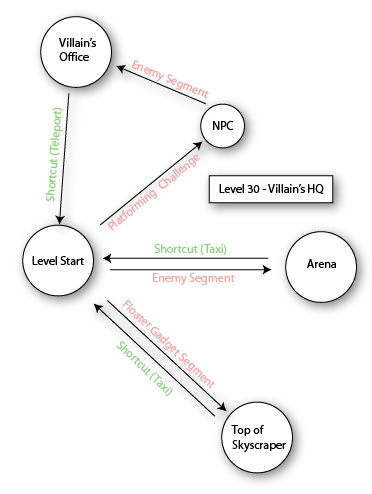
\includegraphics[width=7cm]{Images/bubblediagram.jpg}
		\vspace{0.5cm}
		\caption{Lưu đồ bong bóng}
	\end{figure}
	\hspace*{1cm} 
	\item \textbf{Tạo ra bản sơ lược của màn chơi}\\
	\hspace*{1cm}  Ở giai đoạn này, những nhà thiết kế màn chơi sẽ bắt đầu thiết kế một bản sơ lược cho màn chơi. Các bản thiết kế này có thể là thiết kế ở trên giấy, các phần mềm đồ hoạ như Adobe Illustrator hay
	trực tiếp trên các game engine như Unity, Unreal, ... Với mỗi node trong đồ thị tương ứng với một zone, một room, ta sẽ sắp xếp thứ mà người chơi sẽ phải gặp trong zone đó, đó có thể là quái vật, rương thưởng, hoặc quái vật giả rương thưởng, hoặc các câu đố đòi hỏi người chơi phải giải quyết được mới được tính là clear.  Ngoài ra, họ sẽ nghĩ đến phương pháp để kết nối các zone với nhau dựa theo mũi tên của đồ thị bong bóng cũng như điều kiện trên đó (nếu có).\\
	\hspace*{1cm} Để một màn chơi tổng thể hấp dẫn, dựa theo nhiều trò chơi khác đã thành công trên thị trường, mỗi zone liên tiếp nhau nên có độ khó tăng dần lên. Việc việc mỗi zone tăng dần độ khó như vậy sẽ luôn tạo cho người chơi các thách thức để họ vượt qua. Từ đó, trò chơi sẽ gia tăng trải nghiệm chơi game của người chơi.\\
	\hspace*{1cm} Nếu muốn di chuyển sang vùng kế tiếp thì phải clear vùng hiện tại. Ví dụ, phải clear được vùng 1 thì mới có thể đi đến vùng 2.  Vùng cuối cùng (hoặc điểm cuối cùng trên lưu đồ) sẽ là nơi được đặt một con quái vật boss hoặc mini-boss, nếu clear được thì sẽ được phần thưởng của màn chơi đó.\\
	\hspace*{1cm} Trong giai đoạn này, một vài thông số của màn chơi như diện tích, chiều cao, khoảng cách có thể chưa cố định. Người thiết kế và các lập trình viên sẽ kiểm thử và căn chỉnh dần cho phù hợp với ý đồ của nhà thiết kế.\\
	\item \textbf{Hoàn thành thiết kế màn chơi}\\
	\hspace*{1cm} Đây là giai đoạn cuối cùng, người thiết kế màn chơi sẽ hoàn thành màn chơi từ thiết kế sơ bộ ở giai đoạn 4.\\
	\hspace*{1cm} Người thiết kế màn chơi sẽ kết nối các vùng của màn chơi với nhau. Ở những vùng có thể di chuyển qua lại với nhau, đó có thể đơn giản chỉ là một cánh cổng hay đường hầm. Ở MeowSQL Knight, việc di chuyển 2 vùng khác nhau là tự nhiên, tuy nhiên để di chuyển cần phải clear zone hiện tại.\\
	\hspace*{1cm} Các zone phải được liên kết mới nhau sao cho phải với mỗi node có ít nhất một đường đi từ node bắt đầu, đi qua node hiện tại và đến node kết thúc. Nghĩa là không được có đường cùng trong màn chơi.\\
	\hspace*{1cm} Sau khi hoàn thành thiết lập toàn bộ bản đồ và kiểm thử, các thông số có thể thay đổi được ở giai đoạn 4 phải được thiết lập cố định lại.
\end{enumerate}
\subsubsection{Một số mẹo khi thiết kế màn chơi}
\hspace*{1cm}  Khi thiết kế một màn chơi, có một số mẹo chúng ta có thể tham khảo để kết quả đạt được tốt hơn.
\begin{itemize}
	\item \textbf{Thiết kế có mục đích rõ ràng: } Mỗi màn chơi phải có một mục đích tại sao nó lại tồn tại. Nó có thể là để người chơi học tập cách sử dụng một cơ chế nào đó của trò chơi và luyện tập các cơ chế đã học hoặc giúp cho cốt truyện được làm rõ và đưa đến người chơi. Ở một số trò chơi có cốt truyện, một vài màn chơi có đóng vai trò mở rộng cốt truyện ra.\\
	Từ các mục đích ban đầu, người thiết kế màn chơi phải luôn tập trung thiết kế để phục vụ mục đích đó. Tránh tập trung vào quá nhiều mục tiêu rời rạc, tránh làm level bị nhồi nhét quá nhiều. Điều này sẽ làm người chơi không bị choáng ngợp vì có quá nhiều thứ diễn ra trong màn chơi. Nếu vẫn muốn màn chơi có nhiều mục đích, hãy chắc chắn nó hợp với nhau và không làm cho màn chơi bị rối
	\item \textbf{Tập trung vào tính thực tế và sự đắm chìm khi chơi: } Tính thực tế cũng rất quan trọng và không nên xem nhẹ. Dù bối cảnh có là thế nào, viễn tưởng hoặc huyền ảo thế nào cũng nên thiết kế màn chơi sao cho người chơi cảm thấy vẫn có tính thực tế trong đó. Điển hình là trọng lực, dù cho nhân vật ở trong bất cứ thế giới game nào, thì cũng luôn bị trọng lực tác động vào. Ở các trò chơi bắn súng, người chơi thường thích việc nhà phát hành làm nó trông thực tế nhất có thể, bao gồm trọng lượng súng ảnh hưởng đến tốc độ di chuyển và độ giật khi bắn, độ giật của súng khác nhau, cũng như độ rơi của đạn khi bắn tầm xa. Trong các game về bóng đá, người chơi sẽ quan tâm đến logic trái bóng và cầu thủ trong các tình huống, đặc biệt là các tình huống nguy hiểm trong vòng cấm.\\
	\begin{figure}[H]
		\centering
		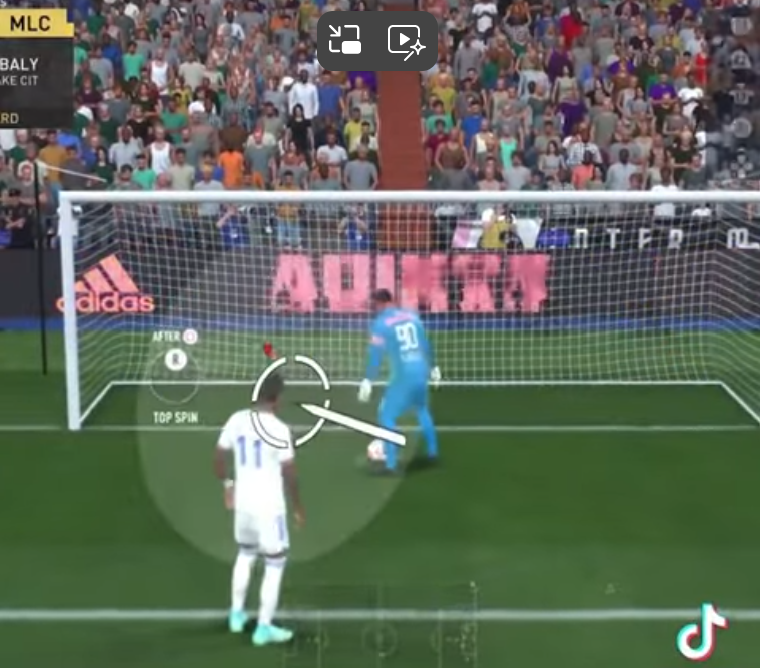
\includegraphics[width=7cm]{Images/FIFAGlitch.png}
		\vspace{0.5cm}
		\caption{Một tình huống penalty phi thực tế trong game}
	\end{figure}
	Nếu áp dụng các yếu tố thực tế một cách hợp lý, người chơi cảm nhận được sự thực tế trong trò chơi. Dần dần, họ bắt đầu chìm đắm vào trò chơi. Việc đắm chìm vô cùng quan trọng, nó cho thấy xu hướng yêu thích và sẽ gắn bó với nó lâu dài. Khi người chơi đã bắt đầu chìm đắm trong trò chơi, họ sẽ bắt đầu quan tâm đến các khía cạnh khác của trò chơi như cốt truyện, đồ hoạ, âm thanh,...
	\item \textbf{Một thử thách không quá dễ dàng nhưng không khó chịu: } Một màn chơi mang tính thử thách hoàn toàn khác với màn chơi khó đến mức gây khó chịu.\\
	Người chơi thích chơi game bởi vì tính thử thách của nó. Các thử thách này sẽ gây khó dễ cho người chơi, đòi hỏi sự rèn luyện, cùng với một khao khát mãnh liệt để vượt qua. Khi đã vượt qua được thử thách, một lượng dopamine được sinh ra khiến người chơi có cảm giác sảng khoái, khiến họ muốn tiếp tục vượt qua thử thách kế tiếp. Đây chính là mục đích cuối cùng mà các màn chơi muốn mang đến cho người chơi. Với dạng trò chơi mang tính chiến thuật như các game bóng đá, đôi khi trò chơi sẽ có một vài màn chơi khó, việc sử dụng một đội hình cố định có thể gặp khó khăn, đòi hỏi phải thay đổi chiến thuật như sử dụng cầu thủ khác, đổi sơ đồ đội hình sao cho qua được màn chơi. Người chơi sẽ cần thử nhiều loại đội hình. Đến một lúc nào đó, họ sẽ tìm ra một đội hình để vượt qua được màn chơi.\\
	Tuy nhiên, đôi khi những người thiết kế màn chơi không tránh khỏi việc trở thành một màn chơi gây khó chịu. Người thiết kế màn chơi đôi khi suy nghĩ rằng chỉ cần đưa hết tất cả những thứ khó nhất vào màn chơi sẽ làm màn chơi mang tính thách thức, hoặc họ nghĩ rằng họ có thể "bào tiền" từ người chơi thông qua các vật phẩm mua bằng tiền thật có thể giúp người chơi qua màn. Nhưng cách này có thể sẽ phản tác dụng. Nhiều trò chơi đã làm theo hướng này và gặp phải tình trạng tỉ lệ User Retention (tỉ lệ người chơi chơi tiếp) giảm đáng kể. Họ tăng độ khó các màn chơi lên rất nhiều, khiến cho việc một người chơi rèn luyện thông thường trong rất lâu để vượt qua nó trở nên bất công so với người chơi chỉ cần bỏ tiền thật để mua một vật phẩm trong cửa hàng, họ có thể dễ dàng vượt qua nó. Đây là một trong những cách làm tồi tệ, có thể giết chết tựa game của mình.\\
	Lấy ví dụ điển hình như trò chơi \textbf{Plants vs. Zombies 2}. Do là trò chơi miễn phí nên lợi nhuận thu được từ các vật phẩm trong game. Ở các phần đầu tiên sẽ xoay quanh việc người chơi xây dựng đội hình tối ưu, học các khả năng của cây mới để tiêu diệt các loại zombies mới, cũng như đi sâu trong chế độ endless mode đầy thử thách. Nếu biết tận dụng cây tốt có thể vượt qua dễ dàng. Trò chơi đón nhận được tình cảm rất lớn từ người chơi. Nhưng sang đến phần 2, nó là một nỗi thất vọng, rồi phần 3 là một thất bại ê chề, khiến cho phần game phải tái phát hành nhiều lần. Điểm mới đầu tiên là một số cây phải mua mới được sử dụng, và độ khó tăng lên nhưng nếu người chơi vận dụng tốt thì vẫn có thể phá đảo toàn bộ game. Về sau, nhà phát triển thêm vào hệ thống cấp độ cho cây và người chơi cần nâng cấp chúng. Càng về sau, các loại cây ban đầu gần như vô cùng yếu dù có nâng cấp và trở nên vô dụng. Người chơi gập muôn vàn khó khăn để vượt qua màn chơi. Hơn nữa, số lượng cây trả phí ngày càng nhiều lên. Chỉ cần bỏ tiền ra mua cây hoặc mua gói nâng cấp cho các cây cũ là có thể qua được dễ dàng. Điều này làm mất đi tính chiến thuật của trò chơi, cộng thêm việc không có thêm các map mới người chơi cũng bắt đầu chán ghét và trò chơi trở nên lụi tàn. Trong những năm gần đây,các bản mod của phần 1 do fan tự làm lại được lòng rất nhiều người chơi, do tính thử thách tăng cao, đi kèm với những loại cây mới phù hợp để người chơi vượt qua thử thách.\\
	Một màn chơi không quá khó cũng không nên quá dễ, nó như vẽ đường cho hươu chạy, sẽ khiến người chơi dễ chán nản. Một màn chơi cũng không nên có quá nhiều hướng dẫn chơi hiện lên, việc hiện hướng dẫn chơi cho người chơi đi đúng hướng là tốt, nhưng có quá nhiều lại trở thành vấn đề khi thiết kế màn chơi, người thiết kế có thể để một số chi tiết cho người chơi tự khám phá, khi đó người chơi sẽ cảm thấy thoả mãn vì bản thân đã học được một thứ mới và đã có thể dùng những gì mới học vượt qua thử thách, mang lại sự thoả mãn. Nhìn chung, việc điều chỉnh độ khó màn chơi sẽ phụ thuộc vào đối tượng mà game đang nhắm đến.\\ 
	
\end{itemize}

\subsection{Ngôn ngữ truy vấn SQL}
\subsubsection{SQL là gì?}
\hspace*{1cm} SQL được viết tắt từ Structured Query Language, là một ngôn ngữ lập trình phục vụ việc lưu trữ và xử lý thông tin trong cơ sở dữ liệu quan hệ. Cơ sở dữ liệu quan hệ lưu trữ thông tin dưới dạng bảng có các hàng và cột đại diện cho những thuộc tính dữ liệu và nhiều mối quan hệ khác nhau giữa các giá trị dữ liệu. Bạn có thể sử dụng các câu lệnh SQL để lưu trữ, cập nhật, loại bỏ, tìm kiếm và truy xuất thông tin từ cơ sở dữ liệu. Bạn cũng có thể sử dụng SQL để duy trì và tối ưu hóa hiệu suất cơ sở dữ liệu.\\
\hspace*{1cm} Ngôn ngữ truy vấn có cấu trúc (SQL) là một ngôn ngữ truy vấn phổ biến thường được sử dụng trong tất cả các loại ứng dụng. Các nhà phân tích và phát triển dữ liệu tìm hiểu và sử dụng SQL do ngôn ngữ này tích hợp hiệu quả với nhiều ngôn ngữ lập trình khác nhau. Theo ANSI (American National Standards Institute - Viện Tiêu chuẩn Quốc gia Hoa Kỳ), SQL là ngôn ngữ tiêu chuẩn cho các hệ thống quản lý cơ sở dữ liệu quan hệ.
\subsubsection{SQL hoạt động như thế nào?}
\hspace*{1cm} Việc triển khai ngôn ngữ truy vấn có cấu trúc (SQL) liên quan đến một máy chủ xử lý truy vấn cơ sở dữ liệu và trả về kết quả. Quá trình SQL đi qua một số thành phần phần mềm sau:\\
\hspace*{1cm}\textbf{Trình phân tích cú pháp}\\
\hspace*{1cm}Trình phân tích cú pháp bắt đầu bằng cách token hóa hoặc thay thế một số từ trong câu lệnh SQL bằng các ký hiệu đặc biệt. Sau đó, nó sẽ kiểm tra câu lệnh để tìm kiếm những yếu tố sau:
\begin{itemize}
	\item Tính đúng đắn: Trình phân tích cú pháp xác minh rằng câu lệnh SQL tuân theo ngữ nghĩa SQL, hay các quy tắc, đảm bảo tính đúng đắn của câu lệnh truy vấn. Ví dụ: trình phân tích cú pháp kiểm tra xem lệnh SQL có kết thúc bằng dấu chấm phẩy hay không. Nếu thiếu dấu chấm phẩy, trình phân tích cú pháp sẽ trả về lỗi.
	\item Quyền hạn: Trình phân tích cú pháp cũng xác thực rằng người dùng đang chạy truy vấn có quyền cần thiết để thao tác với dữ liệu tương ứng. Ví dụ: chỉ người dùng quản trị mới có quyền xóa dữ liệu.
\end{itemize}

% \hspace*{1cm}Tính đúng đắn\\
% \hspace*{1cm}Trình phân tích cú pháp xác minh rằng câu lệnh SQL tuân theo ngữ nghĩa SQL, hay các quy tắc, đảm bảo tính đúng đắn của câu lệnh truy vấn. Ví dụ: trình phân tích cú pháp kiểm tra xem lệnh SQL có kết thúc bằng dấu chấm phẩy hay không. Nếu thiếu dấu chấm phẩy, trình phân tích cú pháp sẽ trả về lỗi.\\

% \hspace*{1cm}Quyền hạn\\
% \hspace*{1cm}Trình phân tích cú pháp cũng xác thực rằng người dùng đang chạy truy vấn có quyền cần thiết để thao tác với dữ liệu tương ứng. Ví dụ: chỉ người dùng quản trị mới có quyền xóa dữ liệu.\\
\hspace*{0.5cm}\textbf{Công cụ quan hệ}\\
\hspace*{1cm}Công cụ quan hệ, hay bộ xử lý truy vấn, tạo kế hoạch truy xuất, ghi hoặc cập nhật dữ liệu tương ứng theo cách hiệu quả nhất. Ví dụ: công cụ này kiểm tra các truy vấn tương tự, sử dụng lại các phương pháp thao tác dữ liệu trước đó hoặc tạo một phương pháp mới. Công cụ quan hệ viết kế hoạch trong mã byte, một dạng biểu diễn trung cấp của câu lệnh SQL. Cơ sở dữ liệu quan hệ sử dụng mã byte để thực hiện tìm kiếm và điều chỉnh cơ sở dữ liệu một cách hiệu quả.\\
\hspace*{1cm}\textbf{Công cụ lưu trữ}\\
\hspace*{1cm}Công cụ lưu trữ, hoặc công cụ cơ sở dữ liệu, là thành phần phần mềm xử lý mã byte và chạy câu lệnh SQL dự định. Công cụ này đọc và lưu trữ dữ liệu trong các tệp cơ sở dữ liệu trên ổ đĩa lưu trữ vật lý. Sau khi hoàn tất, công cụ lưu trữ trả về kết quả cho ứng dụng yêu cầu.
\subsubsection{Các ngôn ngữ truy vấn dữ liệu SQL}
\hspace*{1cm}Lệnh ngôn ngữ truy vấn có cấu trúc (SQL) là những từ khóa hoặc câu lệnh SQL cụ thể được các nhà phát triển sử dụng để thao tác với dữ liệu được lưu trữ trong cơ sở dữ liệu quan hệ. Bạn có thể phân loại các lệnh SQL như sau:\\
\hspace*{1cm}\textbf{Ngôn ngữ định nghĩa dữ liệu}\\
\hspace*{1cm}Ngôn ngữ định nghĩa dữ liệu (DDL) là các lệnh SQL thiết kế cấu trúc cơ sở dữ liệu. Các kỹ sư cơ sở dữ liệu sử dụng DDL để tạo và điều chỉnh các đối tượng cơ sở dữ liệu dựa trên các yêu cầu nghiệp vụ. Ví dụ: kỹ sư cơ sở dữ liệu sử dụng lệnh CREATE để tạo các đối tượng cơ sở dữ liệu như bảng, chế độ xem và chỉ mục.\\
\hspace*{1cm}\textbf{Ngôn ngữ truy vấn dữ liệu}\\
\hspace*{1cm}Ngôn ngữ truy vấn dữ liệu (DQL) bao gồm các lệnh hướng dẫn để truy xuất dữ liệu được lưu trữ trong cơ sở dữ liệu quan hệ. Các ứng dụng phần mềm sử dụng lệnh SELECT để lọc và trả về kết quả cụ thể từ một bảng SQL.\\
\hspace*{1cm}\textbf{Ngôn ngữ thao tác dữ liệu}\\
\hspace*{1cm}Các câu lệnh ngôn ngữ thao tác dữ liệu (DML) viết thông tin mới hoặc điều chỉnh các bản ghi hiện có trong cơ sở dữ liệu quan hệ. Ví dụ: một ứng dụng sử dụng lệnh INSERT để lưu trữ một bản ghi mới trong cơ sở dữ liệu.\\
\hspace*{1cm}\textbf{Ngôn ngữ kiểm soát dữ liệu}\\
\hspace*{1cm}Quản trị viên cơ sở dữ liệu sử dụng ngôn ngữ kiểm soát dữ liệu (DCL) để quản lý hoặc cấp quyền truy cập cơ sở dữ liệu cho người dùng khác. Ví dụ: họ có thể sử dụng lệnh GRANT để cho phép các ứng dụng nhất định thao tác với một hoặc nhiều bảng.\\
\hspace*{1cm}\textbf{Ngôn ngữ kiểm soát giao dịch}\\
\hspace*{1cm}Công cụ quan hệ sử dụng ngôn ngữ kiểm soát giao dịch (TCL) để tự động thực hiện các thay đổi đối với cơ sở dữ liệu. Ví dụ: cơ sở dữ liệu sử dụng lệnh ROLLBACK để hoàn tác một giao dịch bị lỗi.
\begin{figure}[H]
	\centering
	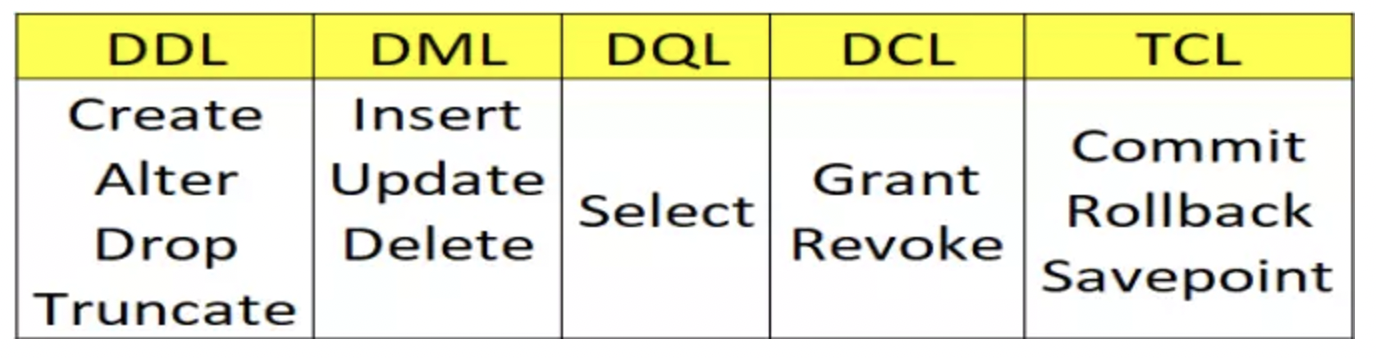
\includegraphics[width=\textwidth]{Images/lệnh SQL.png}
	\vspace{0.5cm}
	\caption{Các câu lệnh SQL cơ bản}
\end{figure}
\subsection{Unity Engine}
Unity là một trong những engine phát triển game phổ biến nhất hiện nay. Unity cung cấp cho người dùng một nền tảng để tạo ra các trò chơi, ứng dụng 2D và 3D một cách thuận tiện và có hệ thống. Ưu điểm của việc sử dụng engine đó là engine sẽ hỗ trợ sẵn những cơ chế cốt lõi của một trò chơi điện tử bao gồm render đồ họa 2D và 3D, tính toán vật lý và va chạm, âm thanh, animation ...\\
Ngôn ngữ lập trình được sử dụng cùng với Unity là C\#. C\# là một ngôn ngữ lập trình thuần hướng đối tượng, rất phù hợp với phát triển hệ thống component-based. Điểm mạnh của C\# là cú pháp tuy đơn giản nhưng rất chặt chẽ và linh hoạt, giúp cho nhà phát triển dễ dàng hiện thực những ý tưởng sáng tạo của mình.\\